\documentclass[14pt]{extbook}
\usepackage{multicol, enumerate, enumitem, hyperref, color, soul, setspace, parskip, fancyhdr} %General Packages
\usepackage{amssymb, amsthm, amsmath, latexsym, units, mathtools} %Math Packages
\everymath{\displaystyle} %All math in Display Style
% Packages with additional options
\usepackage[headsep=0.5cm,headheight=12pt, left=1 in,right= 1 in,top= 1 in,bottom= 1 in]{geometry}
\usepackage[usenames,dvipsnames]{xcolor}
\usepackage{dashrule}  % Package to use the command below to create lines between items
\newcommand{\litem}[1]{\item#1\hspace*{-1cm}\rule{\textwidth}{0.4pt}}
\pagestyle{fancy}
\lhead{Progress Quiz 6}
\chead{}
\rhead{Version A}
\lfoot{1430-1829}
\cfoot{}
\rfoot{test}
\begin{document}

\begin{enumerate}
\litem{
First, find the equation of the line containing the two points below. Then, write the equation as $ y=mx+b $ and choose the intervals that contain $m$ and $b$.\[ (5, 6) \text{ and } (9, -3) \]\begin{enumerate}[label=\Alph*.]
\item \( m \in [0.25, 5.25] \hspace*{3mm} b \in [-23.25, -22.25] \)
\item \( m \in [-7.25, 1.75] \hspace*{3mm} b \in [-20.25, -13.25] \)
\item \( m \in [-7.25, 1.75] \hspace*{3mm} b \in [12.25, 19.25] \)
\item \( m \in [-7.25, 1.75] \hspace*{3mm} b \in [-14, -5] \)
\item \( m \in [-7.25, 1.75] \hspace*{3mm} b \in [-5, 3] \)

\end{enumerate} }
\litem{
Solve the linear equation below. Then, choose the interval that contains the solution.\[ \frac{-5x + 4}{8} - \frac{7x + 9}{4} = \frac{-5x + 5}{6} \]\begin{enumerate}[label=\Alph*.]
\item \( x \in [1, 2.9] \)
\item \( x \in [-1.6, 0] \)
\item \( x \in [-3.4, -1] \)
\item \( x \in [-6.7, -6] \)
\item \( \text{There are no real solutions.} \)

\end{enumerate} }
\litem{
First, find the equation of the line containing the two points below. Then, write the equation as $ y=mx+b $ and choose the intervals that contain $m$ and $b$.\[ (-7, -7) \text{ and } (-2, 6) \]\begin{enumerate}[label=\Alph*.]
\item \( m \in [0.6, 3.6] \hspace*{3mm} b \in [11.08, 12.47] \)
\item \( m \in [0.6, 3.6] \hspace*{3mm} b \in [7.73, 8.62] \)
\item \( m \in [0.6, 3.6] \hspace*{3mm} b \in [-11.83, -10.6] \)
\item \( m \in [-3.6, -0.6] \hspace*{3mm} b \in [0.22, 1.11] \)
\item \( m \in [0.6, 3.6] \hspace*{3mm} b \in [-0.43, 0.11] \)

\end{enumerate} }
\litem{
Write the equation of the line in the graph below in Standard form $Ax+By=C$. Then, choose the intervals that contain $A, B, \text{ and } C$.
\begin{center}
    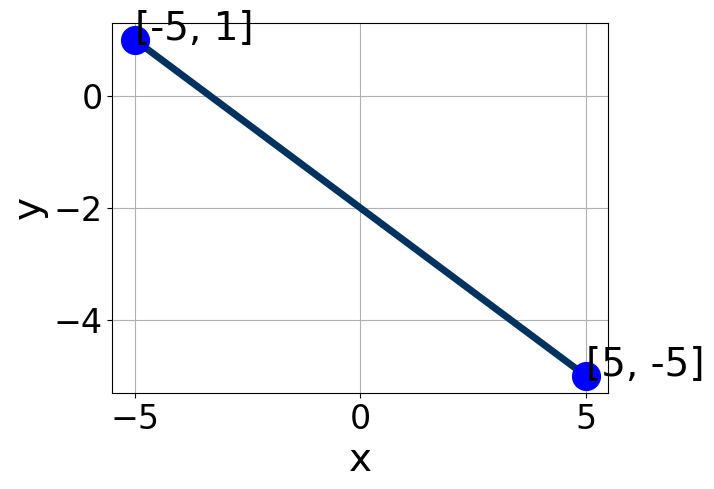
\includegraphics[width=0.5\textwidth]{../Figures/linearGraphToStandardA.png}
\end{center}
\begin{enumerate}[label=\Alph*.]
\item \( A \in [3.7, 4.3], \hspace{3mm} B \in [-5.36, -4.37], \text{ and } \hspace{3mm} C \in [-11.6, -6] \)
\item \( A \in [-4.5, -2.7], \hspace{3mm} B \in [4.57, 5.63], \text{ and } \hspace{3mm} C \in [9.8, 10.9] \)
\item \( A \in [-2.6, 2.8], \hspace{3mm} B \in [0.81, 1.16], \text{ and } \hspace{3mm} C \in [1.3, 2.4] \)
\item \( A \in [3.7, 4.3], \hspace{3mm} B \in [4.57, 5.63], \text{ and } \hspace{3mm} C \in [9.8, 10.9] \)
\item \( A \in [-2.6, 2.8], \hspace{3mm} B \in [-1.28, 0.08], \text{ and } \hspace{3mm} C \in [-3.2, -1.8] \)

\end{enumerate} }
\litem{
Solve the equation below. Then, choose the interval that contains the solution.\[ -2(-4x -9) = -18(-17x + 6) \]\begin{enumerate}[label=\Alph*.]
\item \( x \in [-0.32, -0.25] \)
\item \( x \in [0.26, 0.29] \)
\item \( x \in [0.41, 0.49] \)
\item \( x \in [0.29, 0.32] \)
\item \( \text{There are no real solutions.} \)

\end{enumerate} }
\litem{
Solve the linear equation below. Then, choose the interval that contains the solution.\[ \frac{5x + 8}{4} - \frac{9x -9}{5} = \frac{-7x + 4}{6} \]\begin{enumerate}[label=\Alph*.]
\item \( x \in [-2.7, 0.7] \)
\item \( x \in [-6.8, -3.6] \)
\item \( x \in [-22.9, -18.5] \)
\item \( x \in [-0.8, 2.7] \)
\item \( \text{There are no real solutions.} \)

\end{enumerate} }
\litem{
Solve the equation below. Then, choose the interval that contains the solution.\[ -6(11x -9) = -2(-5x + 13) \]\begin{enumerate}[label=\Alph*.]
\item \( x \in [0.82, 1.15] \)
\item \( x \in [0.46, 0.55] \)
\item \( x \in [0.32, 0.47] \)
\item \( x \in [-0.57, -0.23] \)
\item \( \text{There are no real solutions.} \)

\end{enumerate} }
\litem{
Find the equation of the line described below. Write the linear equation as $ y=mx+b $ and choose the intervals that contain $m$ and $b$.\[ \text{Parallel to } 3 x - 5 y = 6 \text{ and passing through the point } (-10, -8). \]\begin{enumerate}[label=\Alph*.]
\item \( m \in [0.17, 0.84] \hspace*{3mm} b \in [0, 4] \)
\item \( m \in [0.17, 0.84] \hspace*{3mm} b \in [0, 4] \)
\item \( m \in [0.17, 0.84] \hspace*{3mm} b \in [-4, 0] \)
\item \( m \in [0.61, 2.16] \hspace*{3mm} b \in [-4, 0] \)
\item \( m \in [-1.3, -0.37] \hspace*{3mm} b \in [-16, -5] \)

\end{enumerate} }
\litem{
Write the equation of the line in the graph below in Standard form $Ax+By=C$. Then, choose the intervals that contain $A, B, \text{ and } C$.
\begin{center}
    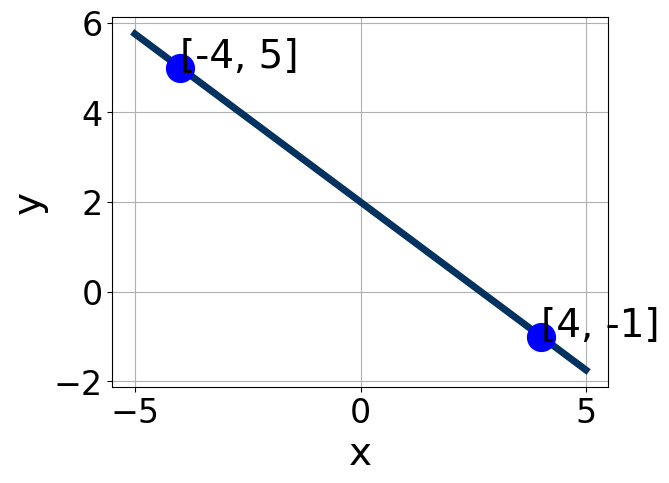
\includegraphics[width=0.5\textwidth]{../Figures/linearGraphToStandardCopyA.png}
\end{center}
\begin{enumerate}[label=\Alph*.]
\item \( A \in [1.6, 7.6], \hspace{3mm} B \in [-3.87, -1.85], \text{ and } \hspace{3mm} C \in [1.66, 3.26] \)
\item \( A \in [-1.2, 2.3], \hspace{3mm} B \in [0.89, 1.98], \text{ and } \hspace{3mm} C \in [-1.4, -0.73] \)
\item \( A \in [-5.5, -0.3], \hspace{3mm} B \in [-3.87, -1.85], \text{ and } \hspace{3mm} C \in [1.66, 3.26] \)
\item \( A \in [1.6, 7.6], \hspace{3mm} B \in [2.08, 4.11], \text{ and } \hspace{3mm} C \in [-3.25, -2.96] \)
\item \( A \in [-1.2, 2.3], \hspace{3mm} B \in [-2.69, -0.15], \text{ and } \hspace{3mm} C \in [-0.34, 1.79] \)

\end{enumerate} }
\litem{
Find the equation of the line described below. Write the linear equation as $ y=mx+b $ and choose the intervals that contain $m$ and $b$.\[ \text{Parallel to } 8 x + 7 y = 8 \text{ and passing through the point } (5, 8). \]\begin{enumerate}[label=\Alph*.]
\item \( m \in [-1.47, -1.05] \hspace*{3mm} b \in [2.5, 4.5] \)
\item \( m \in [-1.47, -1.05] \hspace*{3mm} b \in [-13.8, -11.3] \)
\item \( m \in [1.13, 1.25] \hspace*{3mm} b \in [-2.1, 2.6] \)
\item \( m \in [-0.95, -0.62] \hspace*{3mm} b \in [12.3, 16] \)
\item \( m \in [-1.47, -1.05] \hspace*{3mm} b \in [12.3, 16] \)

\end{enumerate} }
\end{enumerate}

\end{document}